\section{107 --- Binary Tree Level Order Traversal II}
Given a binary tree, return the \textit{bottom-up level order} traversal of its nodes' values. (i.e, from left to right, level by level from leaf to root).

For example:
Given binary tree \fcj{[3,9,20,null,null,15,7]},

\begin{figure}[H]
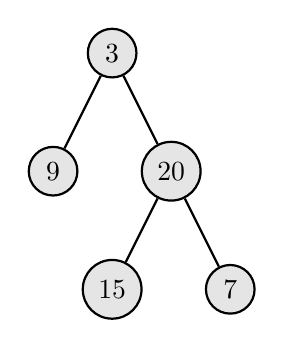
\begin{tikzpicture}
[every node/.style={draw, circle, fill=gray!20!, minimum size=5mm},
%level 1/.style={sibling distance=25mm},
%level 2/.style={sibling distance=15mm},
thick]
\node{3}
child{node{9}}
child{node{20} child{node{15}} child{node{7}}};
\end{tikzpicture}
\end{figure}

return its bottom-up level order traversal as:

\fcj{[ [15,7], [9,20], [3] ]}

\subsection{BFS}
非常容易的题目,用一个queue进行BFS, 然后reverse得到的level遍历数组即可。